\documentclass[11pt]{article}
\usepackage[T1]{fontenc}
\usepackage[utf8]{inputenc}
\usepackage{geometry}
\geometry{verbose,tmargin=1in,bmargin=1in,lmargin=1in,rmargin=1in}
\usepackage{amsmath}
\usepackage{amssymb}
\usepackage{bm}
\usepackage{booktabs}
\usepackage{enumitem}
\usepackage{graphicx}
\setlength{\parskip}{\smallskipamount}
\setlength{\parindent}{0pt}

\input{Macros.tex}

\title{Problem Set 2 --- Solutions\\
\large Labor Economics (Saggio), Summer 2026}
\author{Pablo Fiorentini}
\date{}

\begin{document}
\maketitle

%=======================================================================
\section*{Question 1: Katz and Murphy (1992)}
%=======================================================================

Output is produced with the CES technology
\begin{equation}
F_{t}(H_{t},L_{t})=\Bigl(A_{H_t}H_{t}^{\frac{\sigma-1}{\sigma}}
   +A_{L_t}L_{t}^{\frac{\sigma-1}{\sigma}}\Bigr)^{\frac{\sigma}{\sigma-1}},
\qquad \rho\equiv\frac{\sigma-1}{\sigma}\in(-\infty,1),
\end{equation}
so that the outer exponent is $1/\rho=\sigma/(\sigma-1)$.

\subsection*{Part (a): special cases}

Write $G\equiv A_{H}H^{\rho}+A_{L}L^{\rho}$ and $F=G^{1/\rho}$.

\paragraph{$\sigma\rightarrow0$ ($\rho\rightarrow-\infty$): Leontief.} Suppose $H<L$, so
$H^{\rho}>L^{\rho}$. Factoring the dominant term,
\[
\tfrac1\rho\log G=\log H+\tfrac1\rho\log A_{H}
   +\tfrac1\rho\log\!\Bigl(1+\tfrac{A_{L}}{A_{H}}(L/H)^{\rho}\Bigr)
   \xrightarrow[\rho\rightarrow-\infty]{}\log H,
\]
because $(L/H)^{\rho}\rightarrow0$ and $\tfrac1\rho\log A_{H}\rightarrow0$. Hence
$\boxed{F\rightarrow\min\{H_{t},L_{t}\}}$: high- and low-skill labor are
\emph{perfect complements} and the augmenting terms drop out of the limit.

\paragraph{$\sigma\rightarrow\infty$ ($\rho\rightarrow1$): linear.} The outer exponent
$1/\rho\rightarrow1$ and $\boxed{F\rightarrow A_{H_t}H_{t}+A_{L_t}L_{t}}$: the two skill
groups are \emph{perfect substitutes}.

\paragraph{$\sigma\rightarrow1$ ($\rho\rightarrow0$): Cobb--Douglas.} Using
$A_{H}H^{\rho}=A_{H}e^{\rho\log H}=A_{H}(1+\rho\log H+O(\rho^{2}))$,
\[
\log F=\tfrac1\rho\log\!\bigl(A_{H}+A_{L}\bigr)
  +\frac{A_{H}\log H+A_{L}\log L}{A_{H}+A_{L}}+O(\rho).
\]
The first term diverges unless $A_{H}+A_{L}=1$. Under the natural Katz--Murphy
normalization $A_{H_t}+A_{L_t}=1$ (the weights are shares) it vanishes and
$\boxed{F\rightarrow H_{t}^{A_{H_t}}L_{t}^{A_{L_t}}}$, Cobb--Douglas with
unit elasticity of substitution.

\subsection*{Part (b): the skill premium with inelastic supply}

Treat the quantities $H_t,L_t$ as given (relative supply predetermined) and let
input markets be competitive, so each factor is paid its marginal product.
Differentiating $F=G^{1/\rho}$,
\[
w_{H}=\frac{\partial F}{\partial H}=G^{\frac1\rho-1}A_{H}H^{\rho-1},
\qquad
w_{L}=\frac{\partial F}{\partial L}=G^{\frac1\rho-1}A_{L}L^{\rho-1}.
\]
The common factor $G^{1/\rho-1}$ cancels in the ratio, and using
$\rho-1=-1/\sigma$,
\begin{equation}
\frac{w_{H_t}}{w_{L_t}}=\frac{A_{H_t}}{A_{L_t}}\Bigl(\frac{H_t}{L_t}\Bigr)^{-1/\sigma}
\;\Longrightarrow\;
\boxed{\;\log\omega_{t}=\log\frac{A_{H_t}}{A_{L_t}}-\frac1\sigma\log\frac{H_t}{L_t}\;}
\end{equation}
This is the canonical Katz--Murphy relative-demand equation.
\begin{itemize}[nosep]
\item Skill-biased technical change:
$\dfrac{\partial\log\omega_t}{\partial\log(A_{H_t}/A_{L_t})}=1>0$. A rise in
relative skill-augmenting productivity raises the premium one-for-one.
\item Relative supply:
$\dfrac{\partial\log\omega_t}{\partial\log(H_t/L_t)}=-\dfrac1\sigma<0$. More
skilled labor lowers its relative price; the larger is $\sigma$ (the easier the
substitution), the smaller the depressing effect.
\end{itemize}

\subsection*{Part (c): elastic labor supply}

Now $H_t=H_{0t}w_{H_t}^{\epsilon}$ and $L_t=L_{0t}w_{L_t}^{\epsilon}$, so
\begin{equation}\label{eq:relsupply}
\log\frac{H_t}{L_t}=\log\frac{H_{0t}}{L_{0t}}+\epsilon\,\log\omega_t .
\end{equation}
Substituting the demand relation from (b),
$\log\omega_t=\log\frac{A_{H_t}}{A_{L_t}}-\frac1\sigma\log\frac{H_t}{L_t}$, into
\eqref{eq:relsupply} and solving the resulting fixed point gives
\begin{equation}
\boxed{\;\log\omega_{t}=\frac{\sigma}{\sigma+\epsilon}\,
   \log\frac{A_{H_t}}{A_{L_t}}-\frac{1}{\sigma+\epsilon}\,
   \log\frac{H_{0t}}{L_{0t}}\;}
\end{equation}
\begin{itemize}[nosep]
\item SBTC: $\dfrac{\partial\log\omega_t}{\partial\log(A_{H_t}/A_{L_t})}
=\dfrac{\sigma}{\sigma+\epsilon}\in(0,1)$. The effect is \emph{attenuated}
relative to the inelastic case: a higher premium calls forth more skilled
labor, which partially undoes the wage increase. As $\epsilon\rightarrow0$ we recover
$1$; as $\epsilon\rightarrow\infty$ the premium becomes pinned down by supply and the
effect vanishes.
\item Exogenous relative supply:
$\dfrac{\partial\log\omega_t}{\partial\log(H_{0t}/L_{0t})}
=-\dfrac1{\sigma+\epsilon}$, also attenuated relative to $-1/\sigma$.
\end{itemize}

\subsection*{Part (d): the Katz--Murphy regression}

Let $a_t\equiv\log\frac{A_{H_t}}{A_{L_t}}=\lambda_0+\lambda_1 t+e_t$ and
$s_t\equiv\log\frac{H_{0t}}{L_{0t}}=\psi_0+\nu_t$, with $e_t\perp\nu_t$ i.i.d.,
$\var(e_t)=V_e$, $\var(\nu_t)=V_\nu$. From part (c) the equilibrium objects are
\begin{equation}
y_t\equiv\log\omega_t=\tfrac{\sigma}{\sigma+\epsilon}a_t-\tfrac1{\sigma+\epsilon}s_t,
\qquad
x_t\equiv\log\tfrac{H_t}{L_t}=\tfrac{\epsilon\sigma}{\sigma+\epsilon}a_t
   +\tfrac{\sigma}{\sigma+\epsilon}s_t,
\end{equation}
the second line obtained by inserting $\log\omega_t$ into \eqref{eq:relsupply}.
We run $y_t=\beta_0+\beta_1 t+\beta_2 x_t+u_t$. Because $t$ is included, apply
Frisch--Waugh--Lovell: project everything on $(1,t)$. Since $e_t,\nu_t$ are
i.i.d.\ (orthogonal to $t$), the residualized regressors are
\[
\tilde y_t=\tfrac{\sigma}{\sigma+\epsilon}e_t-\tfrac1{\sigma+\epsilon}\nu_t,
\qquad
\tilde x_t=\tfrac{\epsilon\sigma}{\sigma+\epsilon}e_t+\tfrac{\sigma}{\sigma+\epsilon}\nu_t .
\]
With $\cov(e,\nu)=0$,
\[
\cov(\tilde y,\tilde x)=\tfrac{\sigma}{(\sigma+\epsilon)^2}(\sigma\epsilon V_e-V_\nu),
\qquad
\var(\tilde x)=\tfrac{\sigma^2}{(\sigma+\epsilon)^2}(\epsilon^2 V_e+V_\nu),
\]
so that
\begin{equation}
\boxed{\;\beta_2=\frac{\sigma\epsilon V_e-V_\nu}{\sigma\,(\epsilon^2 V_e+V_\nu)}\;}
\end{equation}
For the trend coefficient, match the deterministic ($t$) parts of $y_t$ and
$x_t$, whose slopes are $g_y=\tfrac{\sigma}{\sigma+\epsilon}\lambda_1$ and
$g_x=\tfrac{\epsilon\sigma}{\sigma+\epsilon}\lambda_1$. Since
$g_y=\beta_1+\beta_2 g_x$,
\[
\beta_1=g_y-\beta_2 g_x
   =\frac{\sigma\lambda_1}{\sigma+\epsilon}\bigl(1-\epsilon\beta_2\bigr)
   =\frac{\sigma\lambda_1}{\sigma+\epsilon}\cdot
    \frac{(\sigma+\epsilon)V_\nu}{\sigma(\epsilon^2V_e+V_\nu)},
\]
which simplifies to
\begin{equation}
\boxed{\;\beta_1=\frac{V_\nu}{\epsilon^2 V_e+V_\nu}\,\lambda_1\;}
\end{equation}

\paragraph{Special cases.}
\begin{center}
\begin{tabular}{lcccl}
\toprule
Case & & $\beta_2$ & $\beta_1$ & \\
\midrule
(a) $\epsilon=0$ (inelastic supply) & & $-1/\sigma$ & $\lambda_1$ & demand identified\\
(b) $V_e=0$ (deterministic tech)    & & $-1/\sigma$ & $\lambda_1$ & demand identified\\
(c) $V_\nu=0$ (no supply shocks)    & & $1/\epsilon$ & $0$ & supply identified\\
\bottomrule
\end{tabular}
\end{center}
Thus $\beta_2=-1/\sigma$ \emph{and} $\beta_1=\lambda_1$ in exactly the same two
cases: (a) and (b). In case (c) the regression instead traces out the
\emph{supply} curve, returning $1/\epsilon$ and a zero trend.

\paragraph{Intuition.} The relative-wage equation is one half of a
simultaneous system. OLS of $\log\omega$ on $\log(H/L)$ recovers the
slope of the demand curve, $-1/\sigma$, only if the variation in relative
\emph{quantities} (after detrending) is driven by supply shifts rather than by
demand (technology) shifts. That happens when (a) supply does not respond to
wages ($\epsilon=0$), so observed quantities are exogenous; or (b) technology
contains no idiosyncratic shocks beyond the smooth trend ($V_e=0$), so the
trend $t$ absorbs all of demand and the residual quantity movements are pure
supply shifts that act as instruments. When instead $V_\nu=0$ and
$\epsilon,V_e>0$, all quantity fluctuations come from demand shocks, and OLS
identifies the supply slope $1/\epsilon$ with $\beta_1=0$.

\subsection*{Part (e): are the assumptions plausible?}

The KM regression treats relative supply as if exogenous to the relative-wage
equation, and reads $-1/\sigma$ off $\beta_2$ and the technology trend off
$\beta_1$. From (d) this is legitimate only if either $\epsilon\approx0$ or
$V_e\approx0$:
\begin{itemize}[nosep]
\item $\epsilon\approx0$ is the more defensible assumption. The relative supply
of college vs.\ high-school labor is governed by slow-moving cohort sizes and
schooling decisions taken years earlier; at annual frequency it is close to
\emph{predetermined}. This is, implicitly, what KM rely on.
\item $V_e=0$ (a purely deterministic, smoothly trending demand) is less
believable literally---technology surely receives shocks---but is a reasonable
approximation if those shocks are small relative to supply movements.
\item The real danger is simultaneity: if demand has genuine high-frequency
shocks ($V_e>0$) \emph{and} supply responds to wages ($\epsilon>0$), then
$\beta_2$ is a variance-weighted average of $-1/\sigma$ and $1/\epsilon$ and is
biased \emph{upward} (toward zero/positive), while $\beta_1\neq\lambda_1$.
\end{itemize}
On balance the exercise is informative if one is willing to treat relative
supply as predetermined, but the inference is fragile; this is exactly why the
later literature (Card--Lemieux, Krusell et al., Acemoglu--Autor) enriches the
demand system and instruments relative supply.

%=======================================================================
\section*{Question 2: Skill Aggregation and Skill Prices}
%=======================================================================

Output is
$Q=\bigl(\sum_i A_i\bigr)^{\alpha}\bigl(\sum_i M_i\bigr)^{\beta}
   \bigl(\sum_i A_iM_i\bigr)^{1-\alpha-\beta}$.
Hippies supply $(A,M)=(2,1)$ and Nerds $(A,M)=(1,3)$. With $H$ hippies and $N$
nerds the three aggregates are
\[
\textstyle\sum_iA_i=2H+N,\quad \sum_iM_i=H+3N,\quad
\sum_iA_iM_i=2H+3N,
\]
the last because each hippy contributes $A_iM_i=2$ and each nerd $A_iM_i=3$. So
\begin{equation}
Q=(2H+N)^{\alpha}(H+3N)^{\beta}(2H+3N)^{1-\alpha-\beta}.
\end{equation}

\subsection*{Part (a): returns to scale and elasticity of substitution}

Each aggregate is linear, hence homogeneous of degree $1$ in $(H,N)$, and the
exponents sum to $\alpha+\beta+(1-\alpha-\beta)=1$. Scaling $(H,N)\rightarrow(tH,tN)$
multiplies each factor by $t$ and $Q$ by $t^{1}$: $Q$ is \textbf{CRTS} in
$(H,N)$.

For the elasticity of substitution between the two \emph{types}, write
$P=2H+N$, $R=H+3N$, $S=2H+3N$, $\gamma=1-\alpha-\beta$, and use that for a
linearly homogeneous $Q(H,N)$,
$\sigma_{HN}=\dfrac{Q_HQ_N}{Q\,Q_{HN}}$. With
$\theta_H\equiv\tfrac{Q_H}{Q}=\tfrac{2\alpha}{P}+\tfrac{\beta}{R}+\tfrac{2\gamma}{S}$,
$\theta_N\equiv\tfrac{Q_N}{Q}=\tfrac{\alpha}{P}+\tfrac{3\beta}{R}+\tfrac{3\gamma}{S}$,
and $D\equiv\tfrac{2\alpha}{P^2}+\tfrac{3\beta}{R^2}+\tfrac{6\gamma}{S^2}$, one
finds $Q_{HN}=Q(\theta_H\theta_N-D)$ and therefore
\begin{equation}
\boxed{\;\sigma_{HN}=\frac{\theta_H\theta_N}{\theta_H\theta_N-D}\;}
\end{equation}
This is positive and \emph{finite} (CRTS implies $Q_{HN}>0$, so the denominator
is positive), but it is \emph{not constant}: it varies with the $H/N$ mix, so
$Q$ is not CES in $(H,N)$ even though it is built from perfect-substitute skill
aggregates. Numerically, at $\alpha=\beta=\tfrac13$ it ranges from
$\sigma_{HN}\approx8.3$ at $H=N$ to $\approx14.6$ at $H/N=1/5$ (see
\texttt{ojs\_solve.py}). The economic content: Hippies and Nerds are close, but
imperfect, substitutes, because they carry different \emph{bundles} of the two
underlying skills.

\subsection*{Part (b): wages, marginal products, and skill prices}

Regard $Q$ as a function of the aggregates
$\mathcal A=\sum A_i,\ \mathcal M=\sum M_i,\ \mathcal B=\sum A_iM_i$, with
marginal products (``skill prices'')
\[
p_A=\frac{\partial Q}{\partial\mathcal A}=\frac{\alpha Q}{\mathcal A},\qquad
p_M=\frac{\partial Q}{\partial\mathcal M}=\frac{\beta Q}{\mathcal M},\qquad
p_B=\frac{\partial Q}{\partial\mathcal B}=\frac{(1-\alpha-\beta)Q}{\mathcal B}.
\]
A competitive firm pays each worker their marginal contribution. Adding one
worker of type $(a,m)$ raises $\mathcal A$ by $a$, $\mathcal M$ by $m$, and
$\mathcal B$ by $am$, so
\begin{equation}
w(a,m)=\frac{\partial Q}{\partial H\text{ or }N}=p_A\,a+p_M\,m+p_B\,(a\,m).
\end{equation}
Concretely $w_H=2p_A+p_M+2p_B$ and $w_N=p_A+3p_M+3p_B$.

\paragraph{Case $\alpha+\beta=1$ ($p_B=0$).} The interaction term disappears and
\[
\boxed{\,w(a,m)=p_A\,a+p_M\,m\,}
\]
is \emph{linear} in the worker's skills with prices $p_A,p_M$ common to all
workers. \textbf{Skill prices are well defined}: a worker's wage is the sum of
the quantities of each skill she carries valued at economy-wide prices, and a
hedonic regression of wages on $(A_i,M_i)$ recovers them.

\paragraph{Case $\alpha+\beta<1$ ($p_B>0$).} Now
\[
w(a,m)=p_A\,a+p_M\,m+p_B\,(a\,m),
\]
which is \emph{non-separable}: the marginal return to ability is
$\partial w/\partial a=p_A+p_B\,m$, i.e.\ it depends on how much motivation the
\emph{same} worker also supplies. \textbf{A single price of ``a unit of
ability'' does not exist}---it is complementary with the worker's other skills.

\paragraph{Usefulness of skill prices.} The notion is useful precisely when the
aggregate skill quantities are sufficient statistics for output
($\alpha+\beta=1$, no within-worker complementarity): then wages are linear in
characteristics, hedonic coefficients are interpretable, and statements like
``the price of cognitive skill rose'' (the SBTC narrative) are meaningful. Once
skills are bundled and complementary within individuals ($\alpha+\beta<1$, the
$\sum A_iM_i$ term), the implicit price of a characteristic is worker-specific,
no common skill price exists, and a linear hedonic regression misidentifies it.
This is Rosen's (1983) and Heckman--Scheinkman's (1987) warning about
\emph{bundling}: aggregation into ``skill prices'' is legitimate only under
strong separability of the technology.

%=======================================================================
\section*{Question 3: On-the-Job Search}
%=======================================================================

Time is discrete (months), agents are infinitely lived and risk neutral, and
discount at $\tfrac1{1+r}$. Flow utility is $w-c$ when employed at $w$ and $b$
when searching; offers arrive at rate $\lambda$ in \emph{both} states, jobs are
destroyed at rate $\delta$, and offers are drawn from $F$ (density $f$). Wages
and benefits are paid at the end of the month, hence discounted.

\subsection*{Part (a): reading equation (1)}

\begin{multline*}
U(w)=\underbrace{\tfrac{w-c}{1+r}}_{\text{(i)}}
 +\tfrac{1}{1+r}\underbrace{\lambda(1-F(w))}_{\text{(ii)}}
   \Bigl[\delta V+(1-\delta)\!\!\int_w^\infty\!\! U(\omega)\tfrac{f(\omega)}{1-F(w)}d\omega\Bigr]\\
 +\tfrac{1}{1+r}\underbrace{\bigl(1-\lambda(1-F(w))\bigr)}_{\text{(iii)}}
   \bigl[\delta V+(1-\delta)U(w)\bigr]
\end{multline*}
\begin{itemize}[nosep]
\item \textbf{(i)} End-of-month flow payoff of the current job, $w-c$,
discounted one period.
\item \textbf{(ii)} With probability $\lambda$ an offer arrives, and it is worth
moving for only if it beats the current wage, i.e.\ with probability
$1-F(w)$; the offer $\omega$ is then a draw from $F$ \emph{truncated} to
$\omega>w$ (density $f(\omega)/(1-F(w))$). But the new job must survive into next
period: with probability $\delta$ it is destroyed and the worker falls into
unemployment $V$, with probability $1-\delta$ she enjoys $U(\omega)$.
\item \textbf{(iii)} With the complementary probability she has no acceptable
offer (no offer, or an offer below $w$) and stays put; entering next period her
\emph{current} job is destroyed with probability $\delta$ ($\rightarrow V$) or survives
($\rightarrow U(w)$).
\end{itemize}
Collecting terms (the $\delta V$ pieces have total weight one) gives the compact
form
\begin{equation}\label{eq:A}
U(w)=\frac{w-c}{1+r}+\frac{\delta V}{1+r}
   +\frac{1-\delta}{1+r}\Bigl[\lambda\!\int_w^\infty\!U(\omega)f(\omega)d\omega
      +\bigl(1-\lambda(1-F(w))\bigr)U(w)\Bigr].
\end{equation}

\subsection*{Part (b): the value of unemployment}

An unemployed worker earns $b$ (end of month, discounted), and with probability
$\lambda$ draws an offer that she accepts iff $\omega\ge w^*$. An accepted job
again faces destruction $\delta$ next period; otherwise she remains unemployed
with continuation $V$:
\begin{equation}\label{eq:V}
V=\frac{b}{1+r}+\frac{1}{1+r}\Bigl[\lambda\!\int_{w^*}^{\infty}\!
   \bigl(\delta V+(1-\delta)U(\omega)\bigr)f(\omega)d\omega
   +\bigl(1-\lambda(1-F(w^*))\bigr)V\Bigr].
\end{equation}

\subsection*{Part (c): the reservation wage is $w^{*}=b+c$}

The reservation wage solves $U(w^*)=V$. Evaluate \eqref{eq:A} at $w^*$, set
$U(w^*)=V$, and write $q\equiv\lambda(1-F(w^*))$ and
$J\equiv\lambda\!\int_{w^*}^{\infty}U(\omega)f(\omega)d\omega$:
\[
(1+r)V=(w^*-c)+\delta V+(1-\delta)\bigl[J+(1-q)V\bigr].
\]
Do the same to \eqref{eq:V}:
\[
(1+r)V=b+\delta q V+(1-\delta)J+(1-q)V.
\]
Subtract. The integral $J$ cancels, and the two continuation blocks are
\emph{identical}: $\delta V+(1-\delta)(1-q)V=V(1-q+\delta q)$ on one side and
$\delta qV+(1-q)V=V(1-q+\delta q)$ on the other. What remains is
\[
w^*-c=b\quad\Longrightarrow\quad\boxed{\,w^{*}=b+c\,.}
\]

\paragraph{Intuition and contrast with the no-OJS model.} Search is equally
productive while employed and while unemployed ($\lambda$ is common to both
states), and the destruction risk $\delta$ is the same. Hence the
\emph{option value of future search} and the job-loss risk are identical at
$U(w^*)$ and at $V$, and they cancel: the worker accepts as soon as the flow
payoff of working, $w-c$, covers the flow payoff of unemployment, $b$. In the
basic McCall model \emph{without} on-the-job search, accepting a job forecloses
further search (employment is absorbing), so the reservation wage embeds a
strictly positive option value---$w^*$ exceeds $b$ ($+$disutility) by the
expected gain from sampling better offers,
$w^{*}=b-\nu+\tfrac1r\E[w-w^*\mid w\ge w^*](1-F(w^*))$, and the worker is
``picky.'' With OJS that motive disappears because she keeps the search option
after accepting, collapsing the reservation wage to the static flow comparison
$w^*=b+c$.

\subsection*{Part (d): duration, exit wage, and UI policy}

Each month unemployed the worker exits with probability $q=\lambda(1-F(w^*))$,
so unemployment duration is geometric:
\begin{equation}
\E[\text{duration}]=\frac{1}{\lambda\bigl(1-F(b+c)\bigr)},\qquad
\E[\text{exit wage}]=\E[\omega\mid\omega\ge w^*]
 =\frac{\int_{w^*}^{\infty}\omega f(\omega)d\omega}{1-F(w^*)} .
\end{equation}
Since $w^*=b+c$ is increasing in $b$, a more generous benefit raises both:
\[
\frac{\partial\,\E[\text{duration}]}{\partial b}
 =\frac{f(w^*)}{\lambda(1-F(w^*))^{2}}>0,\qquad
\frac{\partial\,\E[\text{exit wage}]}{\partial b}
 =\frac{f(w^*)}{1-F(w^*)}\bigl(\E[\omega\mid\omega\ge w^*]-w^*\bigr)>0 .
\]
Higher $b$ makes workers choosier, lengthening joblessness but improving the
accepted wage. At the calibration of part (g) ($w^*=800$): $1-F(w^*)=0.841$,
the monthly exit hazard is $0.168$, expected duration is $5.94$ months, and the
expected re-employment wage is $1{,}314$.

\paragraph{Policy.} This is precisely the tension stressed in class around
extending UI (Nekoei--Weber 2017): longer potential benefits raise reservation
wages, increasing both unemployment duration (a moral-hazard / fiscal cost)
\emph{and} re-employment wages (a match-quality benefit). The model rationalizes
the empirical finding that UI extensions can \emph{raise} accepted wages through
selectivity, so the welfare verdict hinges on trading off longer joblessness
against better matches rather than on duration alone.

\subsection*{Part (e): $U(\bar w)$ and $U(w^{*})$ on support $[0,\bar w]$}

At the top wage no better offer can arrive ($1-F(\bar w)=0$), so the search
terms in \eqref{eq:A} vanish:
\[
U(\bar w)=\frac{\bar w-c}{1+r}+\frac{\delta V}{1+r}
   +\frac{1-\delta}{1+r}U(\bar w)
\;\Longrightarrow\;
\boxed{\,U(\bar w)=\frac{\bar w-c+\delta V}{r+\delta}\,.}
\]
Intuitively, the worker at $\bar w$ has no upgrade option, so she simply holds a
job that yields flow $\bar w-c$ and dies at rate $\delta$: the flow is
capitalized at the \emph{effective} discount rate $r+\delta$, plus the value
$\delta V$ of the job-loss contingency.

Using $V=U(w^*)$ in the contraction \eqref{eq:basef} below at $w=w^*$ gives
\[
\boxed{\,U(w^{*})=V=\frac{b}{r}
   +\frac{\lambda(1-\delta)}{r}\!\int_{w^*}^{\bar w}\!\bigl(U(\omega)-V\bigr)f(\omega)d\omega\,.}
\]
The unemployed worker's value is the perpetuity value of the benefit, $b/r$,
plus the \emph{option value of search}: the expected capital gain from climbing
to better jobs, $U(\omega)-V$, weighted by the arrival rate and survival
probability. (Numerically $V=49{,}292$, well above $b/r=40{,}000$.)

\subsection*{Part (f): the slope $U'(w)$ and the picture}

Differentiate \eqref{eq:basef}. Writing
$I(w)=\int_w^{\bar w}(U(\omega)-U(w))f(\omega)d\omega$ one has
$I'(w)=-U'(w)(1-F(w))$, so
\[
U'(w)=\frac{1}{r+\delta}-\frac{\lambda(1-\delta)}{r+\delta}U'(w)(1-F(w))
\;\Longrightarrow\;
\boxed{\,U'(w)=\frac{1}{\,r+\delta+\lambda(1-\delta)(1-F(w))\,}>0.}
\]
Because $1-F(w)$ falls as $w$ rises, the denominator falls and $U'$ rises:
$U$ is \textbf{increasing and convex}. At the top,
$U'(\bar w)=\dfrac{1}{r+\delta}$ (the numerical derivative gives $3.7037=1/0.27$,
matching exactly). The slope is flattest at the bottom,
$U'(0)=1/[r+\delta+\lambda(1-\delta)]$, because there the option to upgrade is
most valuable, so a marginal wage increase is worth comparatively little.

Figure~\ref{fig:q3} plots the solution: $U(w)$ is increasing and convex, while
$V=U(w^*)$ is a horizontal line crossing $U$ at $w^*=b+c=800$. For $w<w^*$,
$U(w)<V$ (the worker rejects); for $w>w^*$, $U(w)>V$ (she accepts).

\begin{figure}[h]
\centering
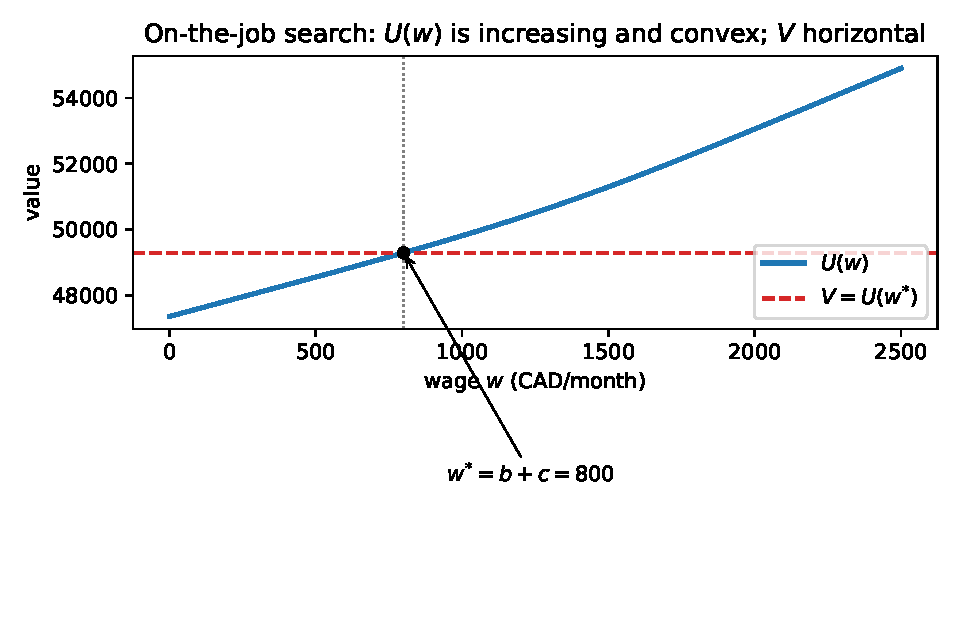
\includegraphics[width=0.74\textwidth]{q3_value_function.pdf}
\caption{Numerical solution of the on-the-job-search model
($b=800,\ c=0,\ \lambda=0.2,\ r=0.02,\ \delta=0.25$, $F=N(1200,400)$,
$\bar w=2500$). $U(w)$ increasing and convex; $V=U(w^*)$ horizontal; they cross
at $w^{*}=b+c=800$.}
\label{fig:q3}
\end{figure}

\subsection*{Part (g): from (1) to the contraction, and the numerical solution}

Substitute $\int_w^{\bar w}U(\omega)f\,d\omega=\int_w^{\bar w}(U(\omega)-U(w))f\,d\omega
+U(w)(1-F(w))$ into \eqref{eq:A}:
\[
U(w)=\frac{w-c}{1+r}+\frac{\delta V}{1+r}+\frac{1-\delta}{1+r}U(w)
  +\frac{\lambda(1-\delta)}{1+r}\!\int_w^{\bar w}\!\bigl(U(\omega)-U(w)\bigr)f(\omega)d\omega .
\]
Move $\tfrac{1-\delta}{1+r}U(w)$ to the left (the coefficient becomes
$\tfrac{r+\delta}{1+r}$), multiply through by $\tfrac{1+r}{r+\delta}$, and use
$V=U(b+c)$:
\begin{equation}\label{eq:basef}
\boxed{\;U(w)=\frac{w-c}{r+\delta}+\frac{\delta\,U(b+c)}{r+\delta}
   +\frac{\lambda(1-\delta)}{r+\delta}\!\int_{w}^{\bar w}\!\bigl(U(\omega)-U(w)\bigr)f(\omega)\,d\omega\;}
\end{equation}
which is the required functional equation $U=T\{U\}$.

\paragraph{Existence/uniqueness.} The algebraically equivalent Bellman map
\eqref{eq:A} places total weight
$\tfrac{\delta}{1+r}+\tfrac{1-\delta}{1+r}\bigl[\lambda(1-F)+(1-\lambda(1-F))\bigr]
=\tfrac{1}{1+r}<1$ on the unknown $U$, so $T$ is a contraction of modulus
$\tfrac1{1+r}$ and has a unique fixed point; successive approximation converges.

\paragraph{Algorithm.} Discretize $[0,2500]$ on a grid of step $1$ (so $w^*=800$
is a node), evaluate $f$ from $N(1200,400)$, and iterate
$U^{n+1}=T\{U^{n}\}$ on \eqref{eq:basef} from $U^{1}(w)=(w-c)/(r+\delta)$ until
$\|U^{n+1}-U^{n}\|_\infty<10^{-9}$, reading $V=U(b+c)$ each pass. The code is in
\texttt{ojs\_solve.py}. It converges in 376 iterations and yields
\[
V=U(800)=49{,}291.6,\qquad U(0)=47{,}357.3,\qquad U(2500)=54{,}899.7 .
\]
Three internal checks confirm the solution: (i) the closed form
$U(\bar w)=(\bar w-c+\delta V)/(r+\delta)$ reproduces $U(2500)$ to the penny;
(ii) iterating the original Bellman form \eqref{eq:A} returns the same $V$ to
within $4\times10^{-8}$; (iii) the numerical $U'(\bar w)=3.7037$ equals
$1/(r+\delta)$.

%=======================================================================
\section*{Question 4: Monopsony and Wage Posting}
%=======================================================================

A monopsonist faces firm-level supply $L(w)$, linear technology, and output
price $P$, with profit $\pi(w)=PL(w)-wL(w)=(P-w)L(w)$ (so the marginal revenue
product of labor is the constant $P$).

\subsection*{Part (a): first-order condition}

\[
\pi'(w)=-L(w)+(P-w)L'(w)=0
\;\Longrightarrow\;
\boxed{\,P-w=\frac{L(w)}{L'(w)}\,}
\;\Longleftrightarrow\;
\frac{P-w}{w}=\frac{1}{\varepsilon_L},\quad
w=\frac{\varepsilon_L}{1+\varepsilon_L}\,P,
\]
where $\varepsilon_L=\dfrac{L'(w)w}{L(w)}$ is the firm's labor-supply
elasticity. The wage is marked down below the marginal product $P$ by the
inverse elasticity---the monopsony wedge.

\subsection*{Part (b): a supply curve that makes profit wage-insensitive}

Require $\pi(w)=(P-w)L(w)=K$ constant. Then
\begin{equation}
\boxed{\,L(w)=\frac{K}{P-w}\,,\qquad w<P,\ K>0.}
\end{equation}
Indeed $\pi(w)=(P-w)\frac{K}{P-w}=K$ for every $w<P$, and one checks
$(P-w)L'(w)=(P-w)\frac{K}{(P-w)^2}=\frac{K}{P-w}=L(w)$, so the first-order
condition holds at \emph{every} wage: the firm is indifferent across the whole
range---the static analogue of Burdett--Mortensen wage dispersion.

\subsection*{Part (c): the implied elasticity}

\[
\varepsilon_L(w)=\frac{L'(w)w}{L(w)}
 =\frac{w/(P-w)^2}{1/(P-w)}=\boxed{\frac{w}{P-w}},
\]
which is \emph{increasing} in $w$: $\varepsilon_L\rightarrow0$ as $w\rightarrow0$ and
$\varepsilon_L\rightarrow\infty$ as $w\rightarrow P$. Higher-wage firms face more elastic supply
(less monopsony power)---directionally plausible. But the specific form is
knife-edge: it requires the elasticity to explode exactly as $w\rightarrow P$, whereas
the empirical literature (e.g.\ Dube et al.\ discussed in class) finds finite,
roughly \emph{constant} firm-level elasticities of order a few. A constant
(isoelastic) supply curve, the usual empirical benchmark, would \emph{not}
deliver wage-insensitive profits. So static wage posting reproduces
Burdett--Mortensen indifference only under a non-robust supply schedule; the
genuine BM result rests on dynamic equilibrium forces, not a single firm's
static supply curve.

\subsection*{Part (d): inverse supply, MFC, demand, and multiplicity}

Inverting (b), $P-w=K/L$, so
\[
w(L)=P-\frac{K}{L}\quad(\text{increasing, concave, }\rightarrow P\text{ as }L\rightarrow\infty),
\]
\[
\text{MFC}=\frac{d}{dL}\bigl[w(L)L\bigr]=\frac{d}{dL}\bigl[PL-K\bigr]=P .
\]
The marginal factor cost is the \emph{constant} $P$, and with linear technology
the inverse labor demand (MRPL) is also the constant $P$. Hence \textbf{MFC and
labor demand coincide} (both horizontal at $P$), while the inverse supply curve
rises toward $P$ from below (Figure~\ref{fig:q4mult}). Because the firm's
marginal benefit of hiring ($P$) equals its marginal cost ($P$) at \emph{every}
employment level, the optimality condition $\text{MFC}=\text{MRPL}$ holds
everywhere: every point on the supply curve is an equilibrium, each delivering
the same profit $K$. The coincidence of the MFC and demand schedules---rather
than a unique crossing---is what generates the continuum of equilibria.

\begin{figure}[h]
\centering
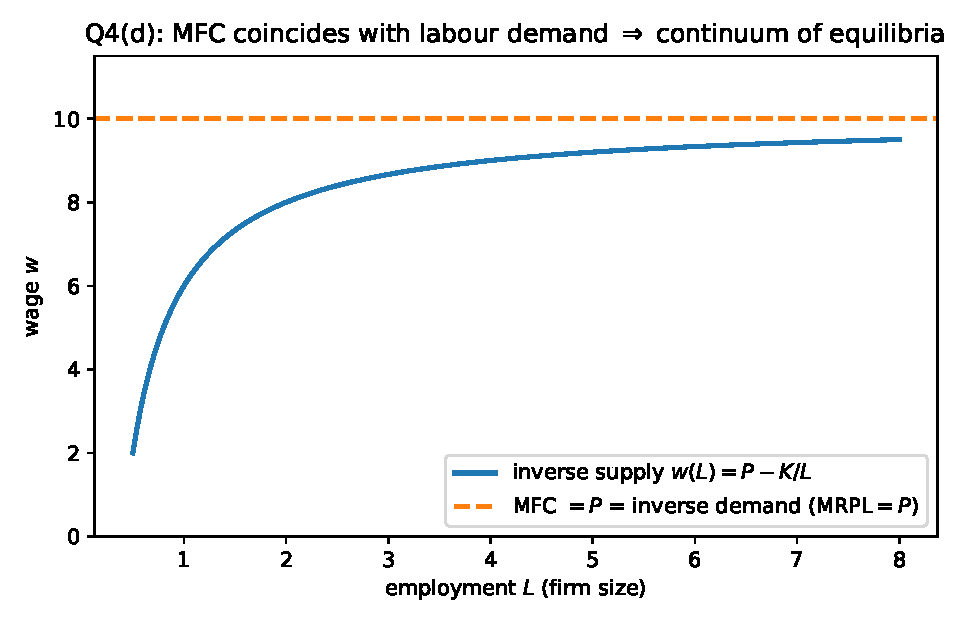
\includegraphics[width=0.66\textwidth]{q4_multiple_equilibria.pdf}
\caption{Inverse supply $w(L)=P-K/L$ rises toward $P$; MFC $=P$ coincides with
inverse labor demand MRPL $=P$. Their overlap (not a unique intersection)
generates a continuum of equilibria.}
\label{fig:q4mult}
\end{figure}

\subsection*{Part (e): a minimum wage at $P/2$}

Start at $w^{*}<P/2$ with employment $L^{*}=K/(P-w^{*})$. Imposing
$w_{\min}=P/2$ (still below $P$, so profit remains $K$ and the firm complies at
exactly $P/2$) moves the firm \emph{up} its supply curve to
\[
L'=\frac{K}{P-P/2}=\frac{2K}{P}>\frac{K}{P-w^{*}}=L^{*}
\qquad(\text{since }w^*<P/2\Rightarrow P-w^*>P/2).
\]
Employment \emph{rises}. This is the classic monopsony result: a minimum wage
set between the posted wage and the marginal product raises wages \emph{and}
employment by moving the firm along an upward-sloping supply curve toward the
competitive point $w=P$ (Figure~\ref{fig:q4min}; at $P=10,K=4$, employment
climbs from $0.571$ to $0.800$).

\begin{figure}[h]
\centering
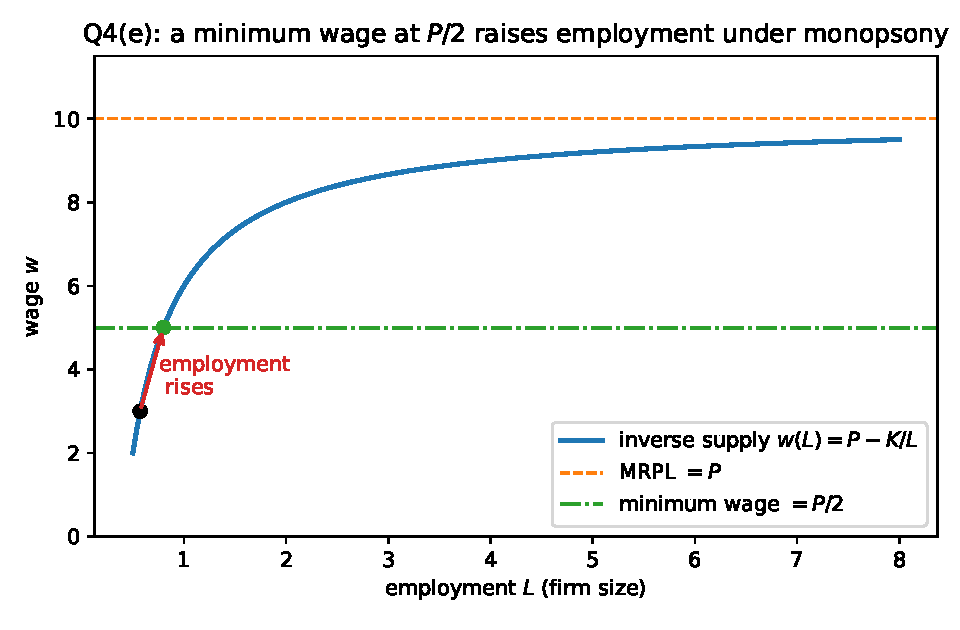
\includegraphics[width=0.66\textwidth]{q4_minimum_wage.pdf}
\caption{A minimum wage at $P/2$ moves the firm up the supply curve from
$(L^*,w^*)$ to $(L',P/2)$: employment increases.}
\label{fig:q4min}
\end{figure}

%=======================================================================
\section*{Question 5: Firm Pay, Amenities, and Compensating Differentials}
%=======================================================================

Worker utility at firm $j$ is $V_j=\log\psi_j+\phi\log a_j$ ($\phi>0$); profit
is $\pi_j=p_j-c_ja_j-\psi_j$; and the firm must deliver at least $\bar V_j$.
Since pay and amenities are costly, the constraint binds,
$\log\psi_j+\phi\log a_j=\bar V_j$.

\subsection*{Part (a): optimal pay and amenities}

The firm minimizes the cost $\psi_j+c_ja_j$ of delivering $\bar V_j$. Tangency
of the iso-utility curve to the iso-cost line gives
$\dfrac{1/\psi_j}{\phi/a_j}=\dfrac{1}{c_j}$, i.e.\ $c_ja_j=\phi\psi_j$. Combining
with the binding constraint,
\begin{equation}
\boxed{\;\log\psi_j=\frac{1}{1+\phi}\bar V_j+\frac{\phi}{1+\phi}\log c_j
   -\frac{\phi}{1+\phi}\log\phi\;}
\end{equation}
\begin{equation}
\boxed{\;\log a_j=\frac{1}{1+\phi}\bar V_j-\frac{1}{1+\phi}\log c_j
   +\frac{1}{1+\phi}\log\phi\;}
\end{equation}
(One verifies $\log\psi_j+\phi\log a_j=\bar V_j$.) Note that productivity $p_j$
does not enter: it is additively separable in profit and so does not affect the
pay/amenity mix chosen to hit $\bar V_j$.

\subsection*{Part (b): common utility $\bar V_j=\bar V$}

With $\bar V_j$ fixed, only $c_j$ varies:
$\log\psi_j=\text{const}+\tfrac{\phi}{1+\phi}\log c_j$ and
$\log a_j=\text{const}-\tfrac{1}{1+\phi}\log c_j$. They are deterministic,
oppositely-signed functions of the single driver $\log c_j$, so
\[
\boxed{\corr(\log\psi_j,\log a_j)=-1.}
\]
\textbf{Intuition.} Holding utility fixed, firms differ only in how cheaply they
can supply amenities. High-$c_j$ firms deliver utility through pay (high $\psi$,
low $a$); low-$c_j$ firms through amenities. This is the pure
\emph{compensating-differentials} trade-off: along an iso-utility locus pay and
amenities substitute one-for-one, producing a perfect negative correlation.

\subsection*{Part (c): common amenity cost $c_j=\bar c$}

Now only $\bar V_j$ varies:
$\log\psi_j=\tfrac{1}{1+\phi}\bar V_j+\text{const}$ and
$\log a_j=\tfrac{1}{1+\phi}\bar V_j+\text{const}$, both increasing in
$\bar V_j$, so
\[
\boxed{\corr(\log\psi_j,\log a_j)=+1.}
\]
\textbf{Intuition.} When the cost of amenities is common but firms differ in the
utility they deliver, high-$\bar V$ firms are simply ``better'': they pay more
\emph{and} offer better amenities. This is \emph{vertical differentiation}---good
firms vs.\ bad firms---and produces a positive pay--amenity correlation, the
opposite of compensating differentials.

\subsection*{Part (d): the general covariance}

Writing $A=\tfrac{1}{1+\phi}$, $\log\psi_j=A\bar V_j+\phi A\log c_j+\text{const}$
and $\log a_j=A\bar V_j-A\log c_j+\text{const}$, so
\begin{equation}
\boxed{\;\cov(\log\psi_j,\log a_j)=\frac{1}{(1+\phi)^2}
  \Bigl[\var(\bar V_j)+(\phi-1)\cov(\bar V_j,\log c_j)-\phi\var(\log c_j)\Bigr].}
\end{equation}
This nests (b) ($\var(\bar V)=0\Rightarrow\cov=-\phi A^2\var(\log c)<0$) and (c)
($\var(\log c)=0\Rightarrow\cov=A^2\var(\bar V)>0$). \textbf{It can be positive}:
whenever firm heterogeneity is dominated by differences in deliverable utility
$\bar V_j$ (vertical differentiation) rather than in amenity costs $c_j$. The
sign is a horse race between the Rosen force (variation in $c_j$, pushing toward
negative correlation) and the firm-quality force (variation in $\bar V_j$,
pushing positive). A positive measured covariance---the empirical pattern that
better-paying firms also have better amenities, and the ``no compensating
differentials'' finding shown in class---therefore does \emph{not} reject
compensating differentials; it merely says firm-quality dispersion outweighs
amenity-cost dispersion.

\subsection*{Part (e): regressing $\log\psi_j$ on $\bar V_j$}

\[
\text{slope}=\frac{\cov(\log\psi_j,\bar V_j)}{\var(\bar V_j)}
 =\frac{1}{1+\phi}\Bigl[1+\phi\,\frac{\cov(\bar V_j,\log c_j)}{\var(\bar V_j)}\Bigr].
\]
It identifies the structural parameter $\tfrac{1}{1+\phi}$ (hence $\phi$)
\emph{only} under the orthogonality assumption $\cov(\bar V_j,\log c_j)=0$:
firms that deliver more utility are not systematically cheaper/dearer at
providing amenities. Otherwise the omitted $\log c_j$ contaminates the slope
(omitted-variable bias) and it identifies no single parameter.

\subsection*{Part (f): the residual variance and ``Rosen motives''}

Let $\hat e_j$ be the residual from the regression in (e). Then
\[
\var(\hat e_j)=\var(\log\psi_j)-\cov(\log\psi_j,\bar V_j)^2/\var(\bar V_j),
\]
which after substitution collapses to
\begin{equation}
\boxed{\;\var(\hat e_j)=\frac{\phi^2}{(1+\phi)^2}
   \Bigl[\var(\log c_j)-\frac{\cov(\bar V_j,\log c_j)^2}{\var(\bar V_j)}\Bigr]
   =\frac{\phi^2}{(1+\phi)^2}\,\var\!\bigl(\log c_j\mid\bar V_j\bigr).}
\end{equation}
\textbf{Interpretation.} The residual is the part of firm pay \emph{not}
explained by the firm's overall utility provision $\bar V_j$---it is the pay
variation driven by differences in the cost of amenities $c_j$ (orthogonal to
$\bar V_j$). Firms with high amenity costs pay more to compensate, for reasons
unrelated to how ``good'' the firm is. This is exactly the
compensating-differential, or \textbf{Rosen-motive}, component of firm pay.

\paragraph{Can one identify the Rosen-motive share?} The share of firm-pay
variance due to Rosen motives is $\var(\hat e_j)/\var(\log\psi_j)$. Computing it
requires (i) data on $\bar V_j$---which is unobserved, but is exactly what Sorkin
(2018) recovers from job-to-job flows via his PageRank/revealed-preference
procedure---and (ii) the orthogonality assumption $\cov(\bar V_j,\log c_j)=0$,
under which firm-pay variance splits cleanly into a vertical-quality piece
(explained by $\bar V_j$) and a compensating-differential piece (the residual).
This is the variance decomposition behind Sorkin's conclusion that roughly half
of firm-pay variation reflects compensating differentials. If instead
$\cov(\bar V_j,\log c_j)\neq0$, the residual captures only the component of
amenity-cost variation orthogonal to firm utility, so $\var(\hat e_j)$ is a
\emph{lower bound} on the true Rosen-motive contribution.

\end{document}
